\chapter[Singular values: Scale factors]{Singular values:\\ Scale factors}

\section{Introduction}
In this chapter we see the singular values\index{singular values!scale factors, as} are called scale factors. Consider the notion of distance. Every point in the domain maps to a point in the codomain. How does the distance between two points in the domain compare to the distance between these two points in the codomain?

%%
\section{Distance}
This section ponders the notion of distance. How do we measure the distance between point in the domain and the codomain. As we saw in the least squares fit, we minimize the distance in the codomain by finding the point nearest to the range of the target matrix $\A{}$. But the solution is a point in the domain. This means that we solve for a point in the codomain and report the solution in the domain.

When we use numeric calculations, we instantly introduce numeric errors. This is a fact of life. Once we introduce errors we are compelled to study the accuracy of our methods. We usually discover that we are not finding an exact answer to our problem. How close is the computed solution $\tilde{x}$ to the exact solution $x$? %(Golub references)\cite[Golub]

There are many details needed to answer this question formally for every algorithm. Here the approach is more intuitive. Suppose we take a step from point $a$ to point $b$ in the domain. These two points map to two points $p$ and $q$ in the codomain. We will see that in general, the distance between these points in not the same:
\begin{equation}
  \dist{a,b} \ne \dist{p,q}.
\end{equation}
In terms of units it is folly to compare the distances as they have different units. For example, in a linear regression the domain is the parameter space of slope and intercept and the codomain is the space of measurements $x$ and $y$. We must measure the separation in the codomain as a displacement in the domain. When we take a step in the domain, we must compare it to another step in the domain induced by a a step in the codomain.

For example, consider the matrix given in %\eqref{}.
\begin{equation}
  a = \otwo, \quad b = \mat{c}{1\\2}.
\end{equation}
The size of the intial step is $\sqrt{3}$.
\begin{equation}
   \begin{split}
     p &= \A{}a = \Aexample \otwo = \othree \\
     q &= \A{}b = \Aexample \mat{c}{1\\2} = \mat{r}{-1\\1\\-1}
  \end{split}.
\end{equation}
The displacement in the codomain is $\sqrt{3}$. The fact that we are comparing distances between \vv \ and \vvv \ should suggest that we need to go back to the world of \vvv s.
\begin{equation}
  \begin{split}
     \hat{a} &= \A{}p = \Atexample \othree = \otwo \\
     \hat{b} &= \A{}q = \Atexample \mat{r}{-1\\1\\-1} = \mat{r}{-3\\3}
  \end{split}
\end{equation}
\begin{equation}
  \begin{split}
     \dist{a,b} &= \sqrt{3} \\
     \dist{\hat{a},\hat{b}} &= \sqrt{18}
  \end{split}
\end{equation}
Money shot
\begin{equation}
  \dist{\hat{a},\hat{b}} = \sqrt{6} \, \dist{a,b} = \sigma_{1} \dist{a,b}
\end{equation}

%%%%
\subsection{Two directions}
Let's do it in two dim.
As you can see from the previous example decompositions, the dimensions of the domain and codomain are not equal in general. We should not expect the distance between two points to be the same as the distance between the two image points. How does the distance between the points in the image
$$ \normt{x_{1} - x_{2}} $$
compare to the distance between the points 
$$ \normt{\A{}x_{1} - \A{}x_{2}}? $$
Start at $x_{1}$, one point in the domain and travel in a straight line to $x_{2}$. We map these points to the codomain as 
\begin{equation}
  \begin{split}
     y_{1} &= \A{}x_{1},\\
     y_{2} &= \A{}y_{2}.
  \end{split}
\end{equation}
Let's pick a matrix that maps from a plane into a plane, $\real{2}\mapsto\real{2}$:
\begin{equation}
  \A{} = \matrixalpha.
\end{equation}
Start at the origin and take a unit step.
The first thing we will discover is that the \emph{direction} of the step affects the length of the step in the codomain:
\begin{equation}
  \A{}e_{1} = \matrixalpha \xhatt = \mat{r}{1\\-1}.
  \label{eq:05:step1}
\end{equation}
In the codomain the distance travelled is this
\begin{equation}
  \normt{ \mat{c}{0\\0} - \mat{r}{1\\-1} } = \sqrt{ 2 }.
\end{equation}
Now take a unit step in the $2-$direction:
\begin{equation}
  \A{}e_{2} = \matrixalpha \yhatt = \mat{r}{2\\2}.
  \label{eq:05:step2}
\end{equation}
In the codomain the distance travelled is this
\begin{equation}
  \normt{ \mat{c}{0\\0} - \mat{c}{2\\2} } = 2.
\end{equation}
The distance travelled depends upon the direction of travel in the domain. Does it depend upon the distance travelled in the domain? Because the matrices are the embodiment of linear operators, we realize that the size of the step does not matter. Let $\alpha$ be an arbitrary scalar:
\begin{equation}
  \A{} \paren{\alpha e_{j}} = \alpha \A{} e_{j}.
\end{equation}

Let's quantify how much the step size changed as we move from domain to codomain. Define
\begin{equation}
\begin{split}
  \Delta x_{j} &= e_{j} - \mat{c}{0\\0} = e_{j}, \\
  \Delta y_{j} &= \A{}e_{j} - \A{}\mat{c}{0\\0} = \A{}e_{j}.
\end{split}
\end{equation}
The dilation factor is given by this
\begin{equation}
  \frac{ \normt{\Delta y_{j}} }{ \normt{e_{}} } = \frac{ \normt{\A{} e_{j}} }{ \normt{e_{j}} } = \normt{\A{} e_{j}}.
\end{equation}

%%%%
\subsection{All directions}
We can look at the behavior as we step in all possible direction. The locus of all possible unit vectors is called the unit circle. We can parameterize this curve with an angular variable $\theta$:
\begin{equation}
  \mathcal{S} = \mat{c}{ \cos \theta \\ \sin \theta }.
\end{equation}
We want to study what happens when the target matrix acts upon this curve:
\begin{equation}
  \A{} \mathcal{S} = \matrixalpha \mat{c}{ \cos \theta \\ \sin \theta } = \mat{r}{ \cos \theta + 2 \sin \theta \\ -\cos \theta + 2 \sin \theta }.
\end{equation}
The result is depicted in figure \eqref{fig:05:steps}. The angular variable is color coded to help the reader see how the coordinate system is rotating.

\begin{figure}[htbp] %  figure placement: here, top, bottom, or page
   \centering
   \includegraphics[ width = 2.25in]{pdf/"ch 05"/"x step"}  \qquad
   \includegraphics[ width = 2.25in]{pdf/"ch 05"/"y step"} \\
   \ \\
   $\A{}\xhatt \quad \to \quad \mat{r}{1\\-1}$ \quad \qquad \qquad \qquad $\A{}\yhatt \quad \to \quad \mat{c}{2\\2}$
   \caption[The matrices in nonsingular decompositions are all square]{Taking steps in domain and the codomain. The inner circle is the unit circle with shading tied to the angular variable. The ellipse is the image of the unit circle under the map $\A{}$. The arrows show the processes in equations \eqref{eq:05:step1} and \eqref{eq:05:step2}. The step in the domain is shown with the solid arrow. The map of this step into the codomain is show with the dashed arrow. We see that the map $\A{}$ dilates the vectors and rotates them. However, the angle between vectors is preserved.}
   \label{fig:05:steps}
\end{figure}

%%%%
\subsection{The return trip}
The previous section served us well as we saw how to measure steps in the domain and the codomain. Now we must complete the round trip from domain to codomain and back to domain. You might think this prudent because in general the spaces have different dimensions. Another reason that we must return to the domain is that different physical meanings the spaces hold. The domain is the space of the fit parameters, for instance slope and intercept in a linear regression. The codomain is the space of measurements. It is meaningless to compare the lengths of a vector in the domain to a vector in the codomain.
\begin{equation*}
  \begin{array}{cccccc}
    domain &\to& codomain &\to& domain \\\hline
    \A{}x_{1} &\to& y_{1} \\ && \A{T}y_{1} &\to& \tildx_{1}
  \end{array}
\end{equation*}
For the scale factors we want to check the total dilation:
\begin{equation}
  \frac{\norm{ \tildx_{1} }}{ \norm{x_{1}} } = \frac{\norm{ \A{T}\A{}e_{1} }}{ \norm{e_{1}} } = \norm{ \A{T}\A{}e_{1} }.
\end{equation}
For the two unit vectors in question, our roundtrip has this effect:
\begin{equation*}
  \begin{array}{ccrccc}
    domain &\to& codomain &\to& domain \\\hline
    \A{}\xhatt &\to& \mat{r}{1\\-1} \\ && \A{T}\mat{r}{1\\-1} &\to& \mat{c}{2\\0}\\\hline
    \A{}\yhatt &\to& \mat{c}{2\\2} \\ && \A{T}\mat{c}{2\\2} &\to& \mat{c}{0\\8}
  \end{array}
\end{equation*}
The final dilation factors are these:
\begin{equation}
  \begin{split}
     \normt{ \A{T}\A{}e_{1} } &= \normt{ \mat{c}{2\\0} } = \sqrt{ 2 },\\
     \normt{ \A{T}\A{}e_{2} } &= \normt{ \mat{c}{0\\8} } = 2\sqrt{ 2 }.
  \end{split}
\end{equation}
These are, of course, the singular values of the matrix $\A{}$:
\begin{equation}
  \sigma \paren{ \A{} } = \sqrt{ 2 } \lst{2, 1}.
\end{equation}
Thus we arrive at a very natural picture of the singular values as scale factors describing the dilations during the round trip between domain and codomain.

\clearpage
\break

\begin{SCfigure}
  \centering
  \includegraphics[ width = 2.5in ]%
    {pdf/"ch 05"/"scale factors steps labels"}% picture filename
  \caption[From the domain to the codomain and back]{From the domain to the codomain and back to the domain. The image of the unit circle under the composite map $\A{T}\A{}$. The circle in the center is the curve $\mathcal{S}\paren{\theta}$, the locus of all unit vectors. The outside ellipse is the figure $\A{T}\A{}\mathcal{S}\paren{\theta}$, the composite map which takes the unit vectors from the domain to the codomain and back to the domain. The angle $\theta$ determines the color of the curve.}
\end{SCfigure}


\clearpage
\break

\begin{SCfigure}
  \centering
  \includegraphics[ width = 2in ]%
    {pdf/"ch 05"/"tall man"}% picture filename
  \caption[From the domain to the codomain and back]{From the domain to the codomain and back to the domain. The image of the unit circle under the composite map $\A{T}\A{}$. The circle in the center is the curve $\mathcal{S}\paren{\theta}$, the locus of all unit vectors. The outside ellipse is the figure $\A{T}\A{}\mathcal{S}\paren{\theta}$, the composite map which takes the unit vectors from the domain to the codomain and back to the domain. The angle $\theta$ determines the color of the curve.}
\end{SCfigure}



\endinput
\section[The column vectors]{The column vectors of the domain matrices}
In this chapter we see the singular values\index{singular values!scale factors, as} are called scale factors. Consider the notion of distance. Every point in the domain maps to a point in the codomain. How does the distance between two points in the domain compare to the distance between these two points in the codomain?
\begin{equation}
  \A{}\X{}_{*,c} = \sigma_{c} \Y{}_{*,c}, \quad c = 1, \rho.
\end{equation}

\endinput
\section{The geometry of the SVD}
The geometry of the \svdl \ provides helpful insights into many problems. We will see the a marvelous depiction of the conditioning to a system. We will also see a clear depiction of the singular values as scale factors.

%%
\subsection{The image of a matrix}
A matrix acts on a vector and produces another vector. Looking at this action on unit vectors is helpful. Consider the locus of all possible unit vectors -  the unit circle. The unit vectors are parameterized as
\begin{equation}
  x_{\theta} = \mat{c}{\cos \theta \\ \sin \theta}, \quad \theta\in[0,2\pi).
\end{equation}

Figure \eqref{fig:maps:both} below shows two plots. The unit circle is the plot of $x_{\theta}$ as $\theta$ varies from 0 to 2$\pi$. The ellipse is the vector showing the action of the target matrix on the unit vectors:
\begin{equation}
  y_{\theta} = \A{}x_{\theta} = \mat{r}{\cos \theta + 2\sin \theta\\-\cos \theta + 2\sin \theta}. 
\end{equation}

The ellipse represents the ``image'' of the target matrix; the action of the matrix on the unit vectors. The context here is a graphical representation. Later we will see this word used in the context of vector space. 

\begin{figure}[htbp] %  figure placement: here, top, bottom, or page
   \centering
   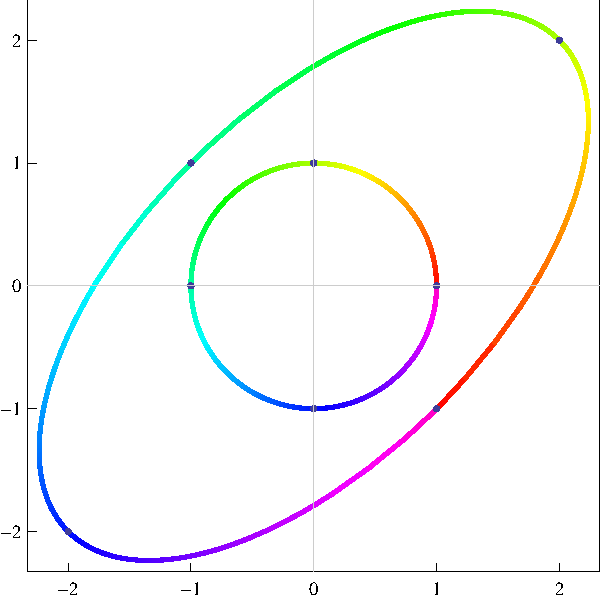
\includegraphics[ width = 2.5in ]{pdf/post_mortemII/dim_22_rank_2_image3} 
   \caption{The mapping action of the matrix in equation \eqref{eq:pmII:A} on all possible unit vectors in $\real{2}$. The coloring of the line is related to the angle. Fiducial marks are shown in increments of $\frac{\pi}{2}$.}
   \label{fig:maps:both}
\end{figure}

The next two plots, in figure \eqref{fig:maps:ev}, separate the curves and adds the eigenvectors. The black arrows are the first eigenvectors and the blue arrows are the second eigenvectors. The unit circle is resolved by the $\X{}$ matrix and the ellipse is resolved by the $\Y{}$ matrix \textit{scaled} by the singular values. This is codified in table \eqref{tab:pmII:blackblue}.

\begin{table}[htdp]
\begin{center}
\boxed{
\begin{tabular}{lrr}
  figure  & blue vector & black vector \\\hline
  circle  & $\X{}_{*,1}$\ \ \ \ \  & $\X{}_{*,2}$\ \ \ \ \  \\
  ellipse & $\sigma_{1} \Y{}_{*,1}$\ \ \ \ \  & $\sigma_{2} \Y{}_{*,2}$\ \ \ \ \ 
\end{tabular}
}
\end{center}
\label{tab:pmII:blackblue}
\caption{The eigenvectors of the domain and codomain and the scaling action of the eigenvectors.}
\end{table}%

This shows the vital relation between the column vectors of the domain and the scaled column vectors of the codomain:
\begin{equation}
  \A{} \X{}_{*,k} = \sigma_{k}\Y{}_{*,k}, \qquad k=1,\rho
  \label{eq:pmII:vital}
\end{equation}
This is of course just a rearrangement of the epitath
$$
\svdax{*}.
$$
The role of the singular values as scale factors is now clear after this demonstration. The blue vectors show the scaling effect of the first singular value; the black vectors the second singular value.

\begin{figure}[htbp] %  figure placement: here, top, bottom, or page
   \centering
   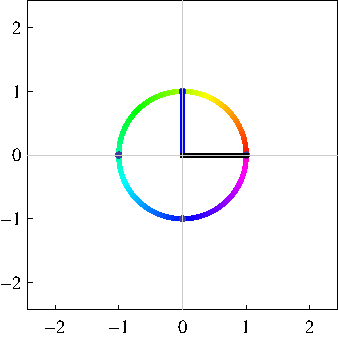
\includegraphics[ width = 2.25in ]{pdf/post_mortemII/circle_ev} \qquad
   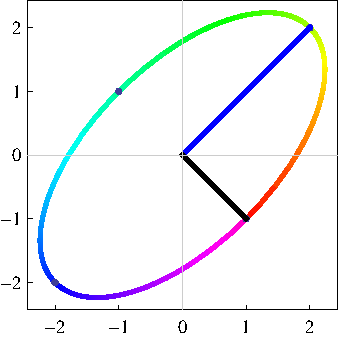
\includegraphics[ width = 2.25in ]{pdf/post_mortemII/ellipse_ev} 
   \caption{The pictorial demonstration of the scaling function of the singular values. The blue vectors show how $\A{} \X{}_{*,1} = \sigma_{k}\Y{}_{*,1}$ and the black vectors show $\A{} \X{}_{*,2} = \sigma_{2}\Y{}_{*,2}$.}
   \label{fig:maps:ev}
\end{figure}

%%
\subsection{The matrix in the simple method}
Look at the map in both directions

%%
\subsubsection{$\A{}x=y$}
\begin{figure}[htbp] %  figure placement: here, top, bottom, or page
   \centering
   \includegraphics[ ]{pdf/post_mortemII/toright} 
   \caption{Examine the mapping action of $\A{}$ from domain to codomain.}
   \label{fig:toright}
\end{figure}

The matrix described in equation \eqref{eq:simple:IamA}.
Recall the first decomposition \eqref{eq:simple:svd}
\begin{equation*}
  \begin{split}
    \svda{T} \\
    \Aexample &= \Yshade \Sigmaexampleb \Xtshade.
  \end{split}
\end{equation*}

Here the rank $\rho=1$ and so there is only one eigenvector to map. The eigenvector $\X{}_{*,1}$ maps to $\sigma_{1}\Y{}_{*,1}$. Since we can't distinctly see the mapping in the 3-dimensional image we show the explicit computation:
\begin{equation}
  \begin{split}
    \A{}\,\X{}_{*,1}\quad &= \quad \sigma_{1}\Y{}_{*,1}, \\
    \Aexample \frac{1}{\sqrt{2}}\mat{r}{1\\-1} \quad & =  \quad \sqrt{6}\frac{1}{\sqrt{3}}\mat{r}{1\\-1\\1}\\
    \frac{2}{\sqrt{2}}\mat{r}{1\\-1\\1}  \quad & =  \quad \sqrt{2}\mat{r}{1\\-1\\1}.
  \end{split}
\end{equation}

Herein lies the problem with the map. The dimension of the image, 1, is less than the dimension of the codomain, 3.

\begin{figure}[htbp] %  figure placement: here, top, bottom, or page
   \centering
   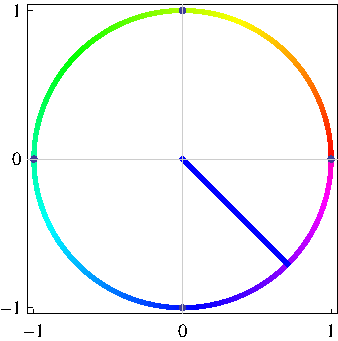
\includegraphics[ width = 1.9in ]{pdf/post_mortemII/a_circle_ev} \qquad
   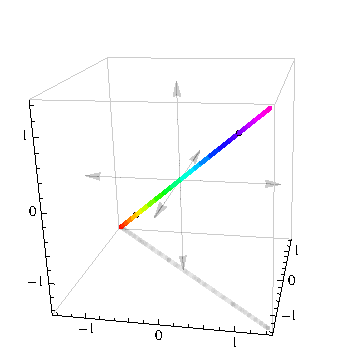
\includegraphics[ ]{pdf/post_mortemII/dim_32_rank_1_image} 
   \caption{The trouble with the matrix $\A{}$ (equation \eqref{eq:simple:IamA}) as a map from domain to codomain. The codomain has dimension 3 yet the image of the target matrix is a line with dimension 1. Because the line is embedded in a $3-$space a point on the line has three coordinates. But along the line there is only one coordinate measuring distance from the origin.}
   \label{fig:toright}
\end{figure}

%%
\subsubsection{$\A{T}y=x$}
\begin{figure}[htbp] %  figure placement: here, top, bottom, or page
   \centering
   \includegraphics[ ]{pdf/post_mortemII/toleft} 
   \caption{Examine the mapping action of the transpose matrix $\A{T}$ from codomain to domain.}
   \label{fig:toright}
\end{figure}
\begin{equation}
  \begin{split}
    \A{T} &= \svdt{T} \\
    \Atexample &= \Xshade \Sigmatexamplea \Ytshade.
  \end{split}
  \label{eq:simple:IamAT}
\end{equation}

\begin{equation}
  \begin{split}
    \A{}\,\X{}_{*,1}\quad &= \quad \sigma_{1}\Y{}_{*,1}, \\
    \Atexample \frac{1}{\sqrt{3}}\mat{r}{1\\-1\\1} \quad & =  \quad \sqrt{6}\frac{1}{\sqrt{2}}\mat{r}{1\\-1}\\
    \frac{3}{\sqrt{3}}\mat{r}{1\\-1}  \quad & =  \quad \sqrt{3}\mat{r}{1\\-1}.
  \end{split}
\end{equation}

\begin{figure}[htbp] %  figure placement: here, top, bottom, or page
   \centering
   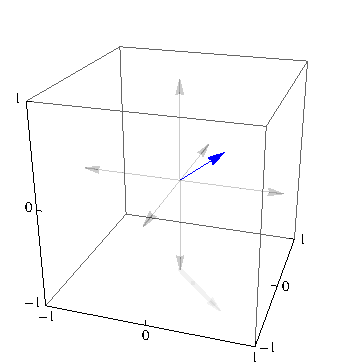
\includegraphics[ ]{pdf/post_mortemII/3_vector}  \qquad
   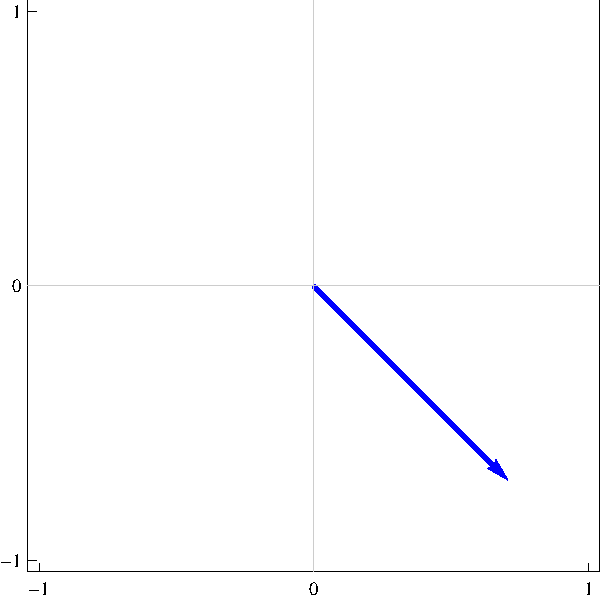
\includegraphics[ width = 1.9in ]{pdf/post_mortemII/430}
   \caption{The trouble with the matrix $\A{T}$ (equation \eqref{eq:simple:IamAT}) as a map from codomain to domain. The codomain has dimension 3 yet the image of the target matrix is a line with dimension 1. Because the line is embedded in a $2-$space a point on the line has two coordinates. But along the line there is only one coordinate measuring distance from the origin.}
   \label{fig:toleft}
\end{figure}

%%
\subsection{The matrix in the general method}
Look at the map in both directions

%%
\subsubsection{Domain $\longrightarrow$ cdomain}
\begin{figure}[htbp] %  figure placement: here, top, bottom, or page
   \centering
   \includegraphics[ ]{pdf/post_mortemII/toright} 
   \caption{Examine the mapping action of $\A{}$ from domain to codomain.}
   \label{fig:toright}
\end{figure}

Start with the first decomposition \eqref{eq:gen:soln}.
\begin{equation}
  \begin{split}
    \A{} &= \Y{}\paren{\sig{}\,\X{T}},\\
     &=
  \frac{1}{\sqrt{2}}
  \mat{rr}{1 & -1\\1 & 1}
  \frac{1}{\sqrt{2}}
  \paren{
  \mat{crc}
  {
  1 & 5  & 2 \\
  1 & -1 & 2
  }}, \\
  &=
  \mat{ccc}
  {
  0 & 3 & 0 \\
  1 & 2 & 2
  }.
  \end{split}
  \label{eq:gen:soln}
\end{equation}

Here the rank $\rho=1$ and so there is only one eigenvector to map. The eigenvector $\X{}_{*,1}$ maps to $\sigma_{1}\Y{}_{*,1}$. Since we can't distinctly see the mapping in the 3-dimensional image we show the explicit computation:
\begin{equation}
  \begin{split}
    \A{}\,\X{}_{*,1}\quad &= \quad \sigma_{1}\Y{}_{*,1}, \\
    \Aexample \frac{1}{\sqrt{2}}\mat{r}{1\\-1} \quad & =  \quad \sqrt{6}\frac{1}{\sqrt{3}}\mat{r}{1\\-1\\1}\\
    \frac{2}{\sqrt{2}}\mat{r}{1\\-1\\1}  \quad & =  \quad \sqrt{2}\mat{r}{1\\-1\\1}.
  \end{split}
\end{equation}

Herein lies the problem with the map. The dimension of the image, 1, is less than the dimension of the codomain, 3.

\begin{figure}[htbp] %  figure placement: here, top, bottom, or page
   \centering
   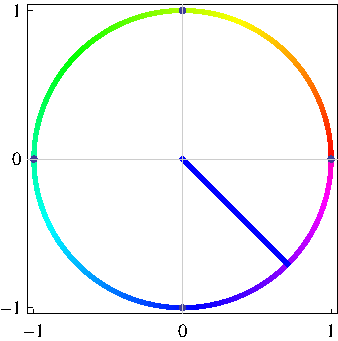
\includegraphics[ width = 1.9in ]{pdf/post_mortemII/a_circle_ev} \qquad
   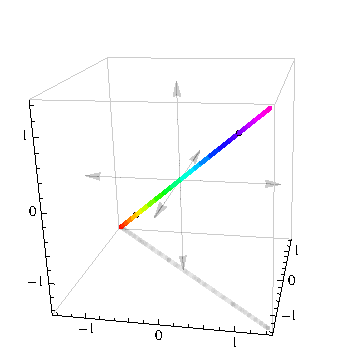
\includegraphics[ ]{pdf/post_mortemII/dim_32_rank_1_image} 
   \caption{The trouble with the matrix $\A{}$ (equation \eqref{eq:simple:IamA}) as a map from domain to codomain. The codomain has dimension 3 yet the image of the target matrix is a line with dimension 1. Because the line is embedded in a $3-$space a point on the line has three coordinates. But along the line there is only one coordinate measuring distance from the origin.}
   \label{fig:toright}
\end{figure}

%%
\subsubsection{$\A{T}y=x$}
\begin{figure}[htbp] %  figure placement: here, top, bottom, or page
   \centering
   \includegraphics[ ]{pdf/post_mortemII/toleft} 
   \caption{Examine the mapping action of the transpose matrix $\A{T}$ from codomain to domain.}
   \label{fig:toright}
\end{figure}
\begin{equation}
  \begin{split}
    \A{T} &= \svdt{T} \\
    \Atexample &= \Xshade \Sigmatexamplea \Ytshade.
  \end{split}
  \label{eq:simple:IamAT}
\end{equation}

\begin{equation}
  \begin{split}
    \A{}\,\X{}_{*,1}\quad &= \quad \sigma_{1}\Y{}_{*,1}, \\
    \Atexample \frac{1}{\sqrt{3}}\mat{r}{1\\-1\\1} \quad & =  \quad \sqrt{6}\,\frac{1}{\sqrt{2}}\mat{r}{1\\-1}\\
    \frac{3}{\sqrt{3}}\mat{r}{1\\-1}  \quad & =  \quad \sqrt{3}\mat{r}{1\\-1}.
  \end{split}
\end{equation}

\begin{figure}[htbp] %  figure placement: here, top, bottom, or page
   \centering
   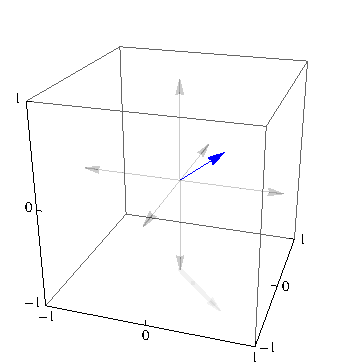
\includegraphics[ ]{pdf/post_mortemII/3_vector}  \qquad
   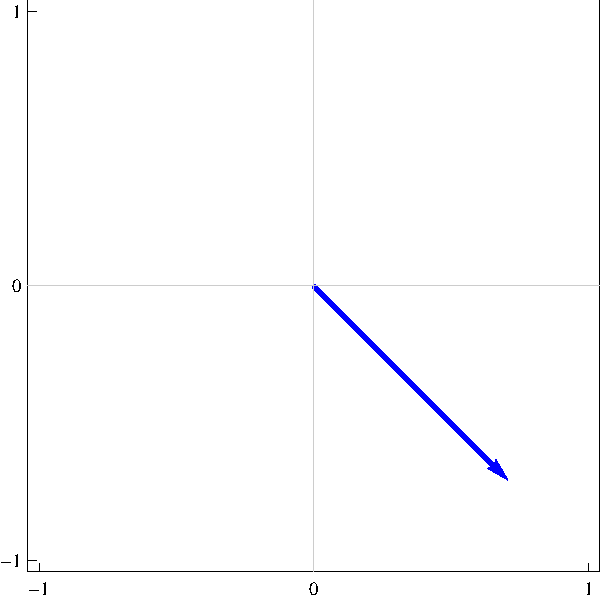
\includegraphics[ width = 1.9in ]{pdf/post_mortemII/430}
   \caption{The trouble with the matrix $\A{T}$ (equation \eqref{eq:simple:IamAT}) as a map from codomain to domain. The codomain has dimension 3 yet the image of the target matrix is a line with dimension 1. Because the line is embedded in a $2-$space a point on the line has two coordinates. But along the line there is only one coordinate measuring distance from the origin.}
   \label{fig:toleft}
\end{figure}


\endinput
\section{A survey of matrix mappings}
In the following pages we will look at three different kinds of mappings for a matrix $\Acc{m}{n}$: no frustration, frustration in one direction, frustration in both directions.

There are two different ways to view frustrated\index{frustration} mappings:
\begin{enumerate}
\item geometric deficiency\index{geometric deficiency} - mapping into a lower dimensional object;
\item algebraic deficiency\index{algebraic deficiency} - rank deficiency in row or column.
\end{enumerate}

In the examples that follow we will see ellipses mapped into other ellipses. These mappings are not frustrated. But once we map into a lower dimensional object, say from the unit sphere onto a line, the map is frustrated. This also means that we can't reverse the map. We can't make a finite linear map from a line with one parameter onto a sphere with three parameters.

These tables specify critical properties of the target matrix.

\textbf{Plots: }All plots start with the unit circle which is either
\begin{equation}
  \begin{array}{rcll}
     S(\theta) &=& \mat{c}{\cos \theta\\\sin \theta},\ \theta\in[0,2\pi) \qquad &n=2,\\
     S(\theta,\phi) &=& \mat{c}{\cos \theta\sin \phi\\\sin \theta \sin \phi\\\cos \phi},\ \theta\in[0,2\pi),\ \phi\in[0,\pi), \qquad &n=3.
  \end{array}
\end{equation}
Then look at the mapping action of the matrix. The result is either
\begin{equation}
  \A{}S(\theta) 
\end{equation}
when the target matrix has two columns or
\begin{equation}
  \A{}S(\theta,\phi) 
\end{equation}
when the target matrix has three columns.

The circles and ellipses have the color determined the the angular variable to provide an clearer idea of how the unit circle is distorted. So for the color red starts at $\theta=0$ and progresses through the spectrum until $\theta=2pi$ where the color is violet.\\

\textbf{Matrix images:} This block summarizes the plot above. For example, it may say that the plot represents a unit sphere being mapped to a line.\\

%%
\textbf{Vector space mappings:} These mappings are based on the dimensions of the spaces for the row and column vectors, $m$ and $n$. They disregard the issue of rank and and concerned purely with the mappings $\real{m}\mapsto\real{n}$ and  $\real{n}\mapsto\real{m}$. This map addresses the geometric deficiency of the mappings. For example are we going from a plane to a plane or a plane to a line. If the map is into a higher dimensional space we will have a frustrated map.\\

\textbf{Matrix ranks:} Are there rank deficiencies in the row or column space? If there is a rank deficiency we will see a frustrated map. 


\clearpage

%%
%% 2 x 2
%%
\begin{table}[htdp]
\begin{center}
\begin{tabular}{cc}
  $\A{}x=y$ & $\A{T}y=x$\\
 $\textellipsis$ & $\textellipsis$ \\
$\mat{rr}{1&2\\-1&2}\mat{c}{x_{1}\\x_{2}} = \mat{c}{y_{1}\\y_{2}}$ &
$\mat{rr}{1&-1\\2&2}\mat{c}{x_{1}\\x_{2}} = \mat{c}{y_{1}\\y_{2}}$ \\
\ \\
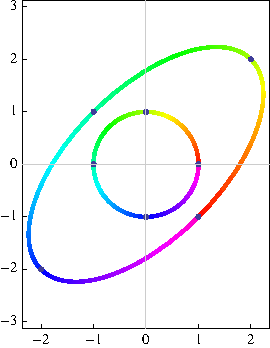
\includegraphics[ width = 2.15in ]{pdf/post_mortemII/2_2_2} &
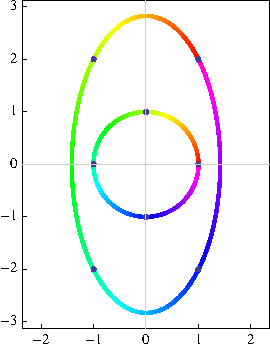
\includegraphics[ width = 2.15in ]{pdf/post_mortemII/2_2_2_t} \\
%%
\ \\
 matrix image & transpose matrix image \\
unit circle $\mapsto$ ellipse & unit circle $\mapsto$ ellipse\\
 $\textellipsis$ & $\textellipsis$ \\
vector space mappings & vector space mappings\\
(Domain) $\real{2} \mapsto \real{2}$ (Codomain) & (Codomain) $\real{2} \mapsto \real{2}$ (Domain)\\
 $\textellipsis$ & $\textellipsis$ \\
 full column rank  & full row rank\\
  $\textellipsis$ & $\textellipsis$ \\
 $\Ap=\AinvL$ & $\Ap=\AinvR$\\[10pt]
\end{tabular}
\end{center}
\label{tab:interpII:a}
\caption{Maps with no frustration. The domain and the codomain have the same dimension and the matrix has full rank. There are no null spaces associated with either the matrix or its transpose. The block dots are fiducial marks to help with comparing the orientation of the image (ellipse) relative to the target (circle). This matrix has full row rank, therefore the pseudoinverse is a left inverse. This matrix has full column rank, therefore the pseudoinverse is a right inverse. Because the pseudoinverse is both a left and a right inverse the pseudoinverse is also the standard inverse.}
\end{table}%

\clearpage
%%
%% 2 x 3
%%
\begin{table}[htdp]
\begin{center}
\begin{tabular}{cc}
  $\A{}x=y$ & $\A{T}y=x$\\
 $\textellipsis$ & $\textellipsis$ \\
$\mat{ccc}{0&3&0\\1&1&2}\mat{c}{x_{1}\\x_{2}\\x_{3}} = \mat{c}{y_{1}\\y_{2}}$ &
$\mat{cc}{0&1\\3&1\\0&2}\mat{c}{y_{1}\\y_{2}} = \mat{c}{x_{1}\\x_{2}\\x_{3}}$ \\
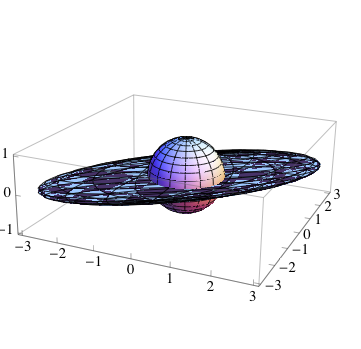
\includegraphics[ width = 2.5in ]{pdf/post_mortemII/3_2_2.png} &
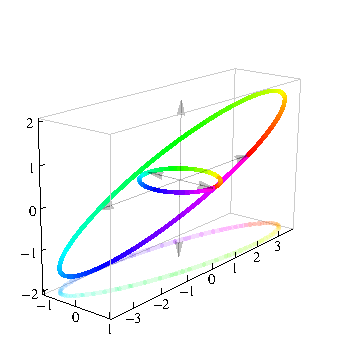
\includegraphics[ width = 2.5in ]{pdf/post_mortemII/3_2_2_t} \\
%%
vector space mappings & vector space mappings\\
(Domain) $\real{3} \mapsto \real{2}$ (Codomain) & (Codomain) $\real{2} \mapsto \real{3}$ (Domain)\\
 $\textellipsis$ & $\textellipsis$ \\
 matrix image & transpose matrix image \\
unit sphere $\mapsto$ elliptic disk & unit circle $\mapsto$ ellipse\\
 $\textellipsis$ & $\textellipsis$ \\
column rank deficient & full row rank\\
frustrated map\\
 $\textellipsis$ & $\textellipsis$ \\
 $\nexists\ \AinvL$ & $\Ap=\AinvR$\\[10pt]
\end{tabular}
\end{center}
\label{tab:interpII:a}
\caption{Frustration in one direction: domain to codomain. The frustration is signaled by the column rank deficiency where the matrix rank is less than the number of columns $(\rho<n)$. Notice that the mapping on the right is not frustrated; it is from a circle to an ellipse. Although both are two-dimensional objects, the ellipse is tipped and tilted out of the plane. The floor of the figure shows a shadow of the ellipse which helps to visualize the orientation in three-space. Because the matrix has full column rank the pseudoinverse is a right inverse.}
\end{table}

\clearpage
%%
%% 3 x 2
%%
\begin{table}[htdp]
\begin{center}
\begin{tabular}{cc}
  $\A{}x=y$ & $\A{T}y=x$\\
 $\textellipsis$ & $\textellipsis$ \\
$\Aexample \mat{c}{x_{1}\\x_{2}} = \mat{c}{y_{1}\\y_{2}\\y_{3}}$ &
$\Atexample\mat{c}{x_{1}\\x_{2}\\x_{3}} = \mat{c}{y_{1}\\y_{2}}$ \\
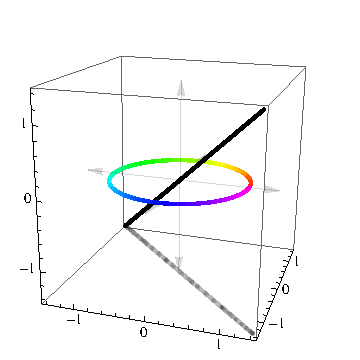
\includegraphics[ width = 2.5in ]{pdf/post_mortemII/3_2_1_a} &
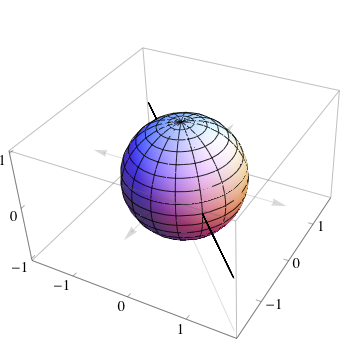
\includegraphics[ width = 2.5in ]{pdf/post_mortemII/3_2_1_t_a} \\
%%
vector space mappings & vector space mappings\\
(Domain) $\real{2} \mapsto \real{3}$ (Codomain) & (Codomain) $\real{3} \mapsto \real{2}$ (Domain)\\
 $\textellipsis$ & $\textellipsis$ \\
 matrix image & transpose matrix image \\
unit circle $\mapsto$ line & unit sphere $\mapsto$ line\\
 $\textellipsis$ & $\textellipsis$ \\
column rank deficient & row rank deficient\\
frustrated map & frustrated map\\
 $\textellipsis$ & $\textellipsis$ \\
 $\nexists\ \AinvL$ &  $\nexists\ \AinvR$ \\[10pt]
\end{tabular}
\end{center}
\label{tab:interpII:c}
\caption{Frustration in both directions, domain to codomain and back. The matrix rank is less than the number of rows $(\rho<m)$ and less than the number of columns $(\rho<n)$. The line is shown in black because the mapping is not one-to-one; multiple points in the target map to the same point in the image. Both figures show a projection of the image onto the floor of the figure. Because the matrix is both column and rank deficient there is neither a left nor a right inverse.}
\end{table}

\endinput

%\input{chapters/"ch 06"/Fourier_Bessel}
%\section{Exercises}
\begin{enumerate}
\item Consider the SVD given for $\Arrr{2}{2}{2}$:
\begin{equation*}
  \svdax{T} = 
  \mat{c|c}{y_{11} & y_{12} \\ y_{21} & y_{22}}
  \mat{cc}{\sigma_{1} & 0 \\ 0 & \sigma_{1}}
  \mat{cc}{x_{11} & x_{12} \\\hline x_{21} & x_{22}}.
\end{equation*}
Show by direct computation of the product that
\begin{equation*}
\begin{split}
  \A{} 
  &= \mat{cc}{
  \sigma_{1} x_{11} y_{11} + \sigma_{2} x_{12} y_{12} & \sigma_{1} x_{21} y_{11} + \sigma_{2} x_{22} y_{12} \\
  \sigma_{1} x_{11} y_{12} + \sigma_{2} x_{12} y_{22} & \sigma_{1} x_{21} y_{12} + \sigma_{2} x_{22} y_{22} } \\
  &= \sigma_{1} \mat{cc}{
  y_{11} \mat{cc}{x_{11} & x_{21}} \\
  y_{12} \mat{cc}{x_{11} & x_{21}}}
  + \sigma_{2} \mat{cc}{
  y_{21} \mat{cc}{x_{12} & x_{22}} \\
  y_{22} \mat{cc}{x_{12} & x_{22}}} \\
  &= \sigma_{1} y_{1}x_{1}^{T} + \sigma_{2} y_{2}x_{2}^{T}.
\end{split}
\end{equation*}
\item
\item
\end{enumerate}


\endinput

\endinput